\documentclass{article}



\usepackage{arxiv}

\usepackage[utf8]{inputenc} % allow utf-8 input
\usepackage[T1]{fontenc}    % use 8-bit T1 fonts
\usepackage{hyperref}       % hyperlinks
\usepackage{url}            % simple URL typesetting
\usepackage{booktabs}       % professional-quality tables
\usepackage{amsfonts}       % blackboard math symbols
\usepackage{nicefrac}       % compact symbols for 1/2, etc.
\usepackage{microtype}      % microtypography
\usepackage{lipsum}		% Can be removed after putting your text content
\usepackage{graphicx}

\usepackage{graphicx, epsfig}
\usepackage[export]{adjustbox}
\usepackage{amsmath, amsthm}
\usepackage{dsfont}
\usepackage{amsfonts}
\usepackage{amssymb}
\usepackage{float}
\usepackage{array}
\usepackage{tikz}
\usepackage{pgfplots}
\usepackage{parskip} 
\usepackage{caption}
\usepackage{float}
\usepackage{xcolor}
\usepackage{placeins}
\usepackage{pdfpages}
\usepackage{framed}
\usepackage{subfigure}

\pgfplotsset{compat=newest} 

\newtheorem{thm}{Theorem}
\newtheorem{lem}{Lemma}
\newtheorem{prop}[thm]{Proposition}
\newtheorem{cor}[thm]{Corollary}
\newtheorem*{claim}{Claim}
\newtheorem{question}{Question}
\theoremstyle{definition}
\newtheorem{defn}[thm]{Definition}
\newtheorem{exam}[thm]{Example}
\newtheorem{problem}[thm]{Problem}
\usepackage{parskip} 
\everymath{\displaystyle}



\let\oldemptyset\emptyset
\let\emptyset\varnothing

\title{Unions of inverse limits of set-valued functions on the unit interval}

%\date{September 9, 1985}	% Here you can change the date presented in the paper title
%\date{} 					% Or removing it

\author{{\includegraphics[scale=0.06]{orcid.png}\hspace{1mm}A. M.~Hankin}
	%% examples of more authors
	\And 
	\href{https://orcid.org/0000-0001-5982-0415}{\includegraphics[scale=0.06]{orcid.png}\hspace{1mm}Robin K. S.~Hankin} \\
	School of Engineering, Computer and Mathematical Sciences\\
	Auckland University of Technology\\
        New Zealand\\
	\texttt{hankin.robin@gmail.com} \\
	%% \AND
	%% Coauthor \\
	%% Affiliation \\
	%% Address \\
	%% \texttt{email} \\
	%% \And
	%% Coauthor \\
	%% Affiliation \\
	%% Address \\
	%% \texttt{email} \\
	%% \And
	%% Coauthor \\
	%% Affiliation \\
	%% Address \\
	%% \texttt{email} \\
}

% Uncomment to remove the date
%\date{}

% Uncomment to override  the `A preprint' in the header
%\renewcommand{\headeright}{Technical Report}
%\renewcommand{\undertitle}{Technical Report}

%%% Add PDF metadata to help others organize their library
%%% Once the PDF is generated, you can check the metadata with
%%% $ pdfinfo template.pdf
\hypersetup{
pdftitle={Unions of inverse limits},
pdfsubject={q-bio.NC, q-bio.QM},
pdfauthor={A. M.~Hankin Robin K. S.~Hankin}
pdfkeywords={Inverse limits},
}

\begin{document}
\maketitle

\newcommand{\invlim}[1]{\lim_{\leftarrow} #1}

\begin{abstract}
We consider set-valued functions from $X=\left[0,1\right]$ to $2^X$
and say that $S = (x_0 , x_1 , x_2 , \ldots)$ is a member of the
inverse limit $\invlim{f}$ of $f\colon X\longrightarrow 2^X$ if $x_i
\in f(x_{i+1})$ for $i = 0, 1, 2, \ldots$.  Given nonempty set-valued
functions $f,g$ with $f$ being onto $X$ (that is, $\forall y\in X,
\exists x\in X\colon y\in f(x)$) and empty intersection (that is,
$\operatorname{Im}(f)\cap\operatorname{Im}(g) = \emptyset$), we prove
that the inverse limit of $f\cup g$ is a strict superset of the union
of the separate inverse limits: $\invlim{f\cap g}
\supset\invlim{f}\cup\invlim{g}$.  We prove a partial converse: for
nonintersecting $f,g$, if $\operatorname{Im}(f)=\left\lbrace
a\right\rbrace$ for some $a\in X$ and $\invlim{f\cup g} =
\invlim{f}\cup\invlim{g$}, then the preimage $g^{-1}(a)=\left\lbrace
a\right\rbrace$.  Further, the idempotence set
$\operatorname{Idem}(f)=\left\lbrace x\colon x\in g(x)\right\rbrace$
is the single element set $\left\lbrace a\right\rbrace$.
\end{abstract}


% keywords can be removed
\keywords{First keyword \and Second keyword \and More}


\section{Definitions}

All functions $f,g,h,\ldots$ are set-valued unless otherwise stated,
with $f\colon X\longrightarrow\mathcal{P}(X)$; here $X=[0,1]$.  We say
that sequence $S = (x_0 , x_1 , x_2 ,\ldots)$ is a member of the
inverse limit of $f\colon X\longrightarrow \mathcal{P}(X)$ if $x_i \in
f(x_{i+1})$ for $i = 0, 1, 2,\ldots$ and write
$S\in\lim_{\leftarrow}f$.  Given two set-valued functions $f,g\colon X
\rightarrow \mathcal{P}(X)$, we define set operators in the usual way,
for example, $(f\cup g)(x) := f(x)\cup g(x)$; we may also compare two
set-valued functions, for example writing $f\subseteq g$ if
$f(x)\subseteq g(x)\forall x\in X$.  We define a {\em partial}
function to be a (set-valued) function whose range includes
$\emptyset$.  Conversely, if the image of every $x\in X$ is nonempty,
$\emptyset\not\in\operatorname{Range}(f)$, we say that $f$ is a {\em
  total} function.  Given a set-valued function $f\colon X
\longrightarrow \mathcal{P}(X)$, we define the {\em graph} $G(f)$ of
$f$ to be $\left\lbrace (x, y) \,|\, x\in X,y \in f(x)\right\rbrace$.
A sequence of the form $( \underbrace{a, a,\ldots, a}_{\text{$n$
    times}}, \underbrace{b, b,\ldots, b}_{\text{$m$ times}},
c,c,\ldots)$ will be denoted $a^nb^mc^\infty$.

\section{Introduction}

We consider the set-valued functions from $X=[0,1]$ to
$\mathcal{P}(X)$ and consider inverse limits in the sense
of~\cite{ingram2012}.  It is intuitive that when we take the union of
two functions, the inverse limit of the resulting function is a
superset of the union of the inverse limits of the two functions:

 \begin{thm}
The inverse limit of $f\cup g$ is a superset of the union of the
inverse limits of $f$ and $g$ separately: $$\invlim{f} \cup \invlim{g}
\subseteq\invlim{f\cup g}$$.
 \end{thm}
 \begin{proof}
If $S = (x_0, x_1, x_2, \ldots)\in\invlim{f}\cup\invlim{g}$ then
either $S\in\invlim{f}$ or $S\in\invlim{g}$.  Thus, for $i\geqslant
0$, $x_i\in f(x_{i+1})\cup g(x_{i+1})$.  So $x_i \in ( f \cup g
)(x_{i+1})$ and so $S\in\invlim{f\cup g}$.
 \end{proof}

This suggests that we consider under what circumstances the inverse
limit of the union is {\em exactly} the union of the inverse limits
with $\invlim{f}\cup\invlim{g} = \invlim{(f\cup g)}$.  We start with
some simple examples.

\begin{exam}
In figure~\ref{abuse}, we have $f(x)=\left\lbrace
a\right\rbrace\,\forall x\in X$ for some $a\in X$ and, with some abuse
of notation,

\begin{equation}
  g(x) = \begin{cases}
    \lbrace a\rbrace & x\leqslant a\\
    \subseteq[0,a) & x>a
    \end{cases}
\end{equation}

(the idea is that $y\in g(x)\longrightarrow y<a$ whenever $x>a$). Then

\begin{equation}
\invlim{f} = \invlim{g} =  \invlim{f \, \cup\, g} = \invlim{f} \,\cup\,
\invlim{g} = a^\infty.
\end{equation}
\end{exam}
\begin{proof}
  It is clear that $\invlim{f}=a^\infty$ and
  also that $a^\infty\in\invlim{g}$.  To prove that $\invlim{f\cup g}=a^\infty$,
  we consider a sequence $(x_0,x_1,\dots)\in\invlim{f\cup g}$ and
  observe that $x_i\leqslant a$ for all $i$.  Further, if $x_i<a$,
  then $x_{i+1}>a$, which is a contradiction.  The result follows from
  theorem 1.
\end{proof}

If, instead, we have

\begin{equation}
  g(x) = \begin{cases}
    \subseteq(a,1] & x<a\\
 a & x\geqslant a
    \end{cases}
\end{equation}

the same result applies, {\em mutatis mutandis}.  However, there are
examples where the inverse limit of the union is a strict superset of 
the union of the inverse limits:

\begin{exam}
Consider
\begin{equation}
  f(x) = \begin{cases}
\lbrace a\rbrace & x\in\lbrace a,b\rbrace\\
\emptyset & \mbox{otherwise}
    \end{cases}\qquad
  g(x) = \begin{cases}
\lbrace b\rbrace & x\in\lbrace a,b\rbrace\\
\emptyset & \mbox{otherwise}
    \end{cases}
\end{equation}

  where we understand $a\neq b$; we could equivalently consider
  $f(x)=\lbrace a\rbrace$ and $g(x)=\lbrace b\rbrace$ for $x\in[0,1]$,
  as shown in figure~\ref{strictly}.  Now $\invlim{f}=a^\infty$ and
  $\invlim{g}=b^\infty$, but $\invlim{f \cup g}$ is precisely
  sequences of the form $(x_0,x_1,x_2,\ldots)$ where $x_i\in\lbrace
  a,b\rbrace$ for $i\geqslant 0$.  The inverse limit of $f\cup g$
  contains $(a,b,\ldots)$ which occurs in neither of the separate
  inverse limits.
\end{exam}

So when is the union of the inverse limits the same as the inverse
limit of the union?  Trivially, if we take two functions (or one
function and a partial function) where one is a subset of the other,
this is the case.  One natural conjecture would be that the inverse
limit of the union of two {\em onto} functions would necessarily be a
strict superset of the union of the inverse limits of the separate
functions.  It is easy to construct such examples:

\begin{exam}
Consider figure~\ref{strictsuperset}.  Here, we have $f(x)=\lbrace
x\rbrace$ and $g(x)=\lbrace 1-x\rbrace$.  Here $\invlim{f}=\lbrace
x^\infty\colon x\in X\rbrace$ and $\invlim{g} = \lbrace (x, 1-x, x,
1-x, \ldots)\colon x\in X\rbrace$.  Writing
$A_S=\lbrace(x_0,x_1,\ldots)\colon x_i\in S\rbrace$, we see that
$\invlim{f\cup g}$ includes $A_{\lbrace x,1-x\rbrace}$ for any $x\in
X$. Thus $\invlim{f\cup
  g}\backslash\left(\invlim{f}\cup\invlim{g}\right)$ is nonempty
including, for example $(1,0,0,\ldots)$.  We see that
$\invlim{f}\cup\invlim{g}$ comprises two arcs that intersect at the
point $0.5^\infty$, whereas $\invlim{f \cup g }$ is a Cantor fan, see
figure~\ref{cantorfan}.
\end{exam}

However, it is possible to construct sets of onto functions for which
the inverse limit of the union is exactly equal to the union of the
inverse limits:

\begin{exam}
Consider

\begin{equation}
  f_U(x) = \begin{cases}
    \lbrace x\rbrace & x\neq a\\
    \lbrace a\rbrace\cup U & x=a
  \end{cases}
\end{equation}

where $U\subseteq X$ is any subset of $X=[0,1]$ and $a\in X$.  Here we
have $\invlim{f_U}=\lbrace x^\infty\colon x\in X\rbrace\cup\lbrace
u^na^\infty\colon u\in U, n\in\mathbb{N}\rbrace$, and also

\begin{equation}
  \bigcup_{i\in I}\invlim{f_{U_i}}=
  \invlim{\bigcup_{i\in I}f_{U_i}}=
  \lbrace x^\infty\colon x\in X\rbrace\cup\lbrace
  u^na^\infty\colon u\in\bigcup_{i\in I}U_i, n\in\mathbb{N}\rbrace.
\end{equation}
\end{exam}

In this case we observe that there is a significant intersection
between the $f_{U_i}$ and indeed $\bigcap_{i\in I}f_{U_i}\supseteq
f\colon x\longrightarrow\lbrace x\rbrace$.  This suggests that pairs
of functions with large overlap (in some sense) have small
$\invlim{f\cup g}\backslash\left(\invlim{f}\cup\invlim{g}\right)$ (in
some sense).  We can formalise a weak version of this suggestion as
follows:

\begin{thm}
If $f$ is onto, $\operatorname{Im}(g)\neq\emptyset$, and $f\cap
g=\emptyset$, then  $\invlim{f\cup g}\supset\invlim{f}\cup\invlim{g}$,
where the set inequality is strict.
\end{thm}

\begin{proof}
The range of $g$ is nonempty, so pick some
$x_0\in\operatorname{im}(g)$.  Then, by definition there must exist
some $x_1$ such that $x_0 \in g(x_1)$.  Then, there must exist some
$x_2$ such that $x_1\in f(x_2)$ since $f$ is onto.  Similarly, there
must be some $x_3$ such that $x_2\in f(x_3)$ and so on.  Then $S=(x_0,
x_1, x_2, x_3\ldots)\not\in\invlim{f}$, for $x_0\not\in f(x_1)$ as
$f\cap g=\emptyset$.  Similarly, $S\not\in\invlim{g}$, for $x_1\not\in
g(x_2)$.
\end{proof}

We now consider unions of a constant function with other functions.
Again define the constant function $f_{U}(\cdot)$ by $f_U(x)=\lbrace
U\rbrace\,\forall x\in X$.  Here we consider unions of $f_{\lbrace
  a\rbrace}$ for some $a\in X$ with a partial function $g$ whose graph
$G(g)$ is a single point:

\begin{equation}
  g(x) = \begin{cases}
    \lbrace c\rbrace & x=b\\
    \emptyset & x\neq b.
    \end{cases}
\end{equation}

(we assume $c\neq a$ throughout, equivalently $g\not\subset f$).  We
know that $\invlim{f_{\lbrace a\rbrace}}=a^\infty$; and

\begin{equation}
  \invlim{g}=\begin{cases}
  b^\infty & b=c\\
  \emptyset &b\neq c
  \end{cases}
\end{equation}


There are three cases:

\begin{itemize}
\item General position: $a\neq b$, $b\neq c$, $c\neq a$.  Then
  $\invlim{f\cup g}=a^\infty$.
\item $a\neq b=c$.  Then $\invlim{f\cup g}=\bigcup_{i\geqslant
  0}b^na^\infty$, a convergent sequence.
\item $a=b\neq c$.  Then
  \begin{multline}
    \invlim{f\cup g}=
    a^\infty\cup
    \lbrace a^nba^\infty|n\in\mathbb{N}\rbrace\\
    \cup\lbrace a^{n_1}ba^{n_2}ba^\infty|n_1\in\mathbb{N},n_2\in\mathbb{N^+}\rbrace
    \cup\cdots\\
    \cdots\cup\lbrace a^{n_1}ba^{n_2}b\ldots a^{n_i}ba^\infty|n_1\in\mathbb{N},n_i\in\mathbb{N}^+,i\geqslant 2\rbrace
    \cup\cdots
  \end{multline}
  Alternatively, we may write
  \begin{multline}
    \invlim{f\cup g}=
    b?a^\infty\cup
    \lbrace b?a^nba^\infty|n\in\mathbb{N^+}\rbrace\\
    \cup\lbrace b?a^{n_1}ba^{n_2}ba^\infty|n_1,n_2\in\mathbb{N^+}\rbrace
    \cup\cdots\\
    \cdots\cup\lbrace b?a^{n_1}ba^{n_2}b\ldots a^{n_i}ba^\infty|n_i\in\mathbb{N}^+\rbrace\cup\cdots
  \end{multline}
  where ``$x?$'' is understood to be either $x^0$ or $x^1$, as in regexp terminology.
  We clearly have $\invlim{f\cup g}\supset\invlim{f}\cup\invlim{g}$.
\end{itemize}

The third case is by far the most interesting (figure~\ref{drawing}).
We note in passing that the inverse limit is not identical to the
underlying set of the finitely presented group $\left\langle
a,b\left|b^2=1\right.\right\rangle$, in which $a$ may have negative
power, unlike the inverse limit in which each $b$ is separated by a
strictly positive power of $a$.

\newcommand{\fa}{f_{\lbrace a\rbrace}}

\begin{thm}\label{fish}
Consider the function $\fa$ for some $a\in X$.  Suppose $g$ is a set
valued function such that $\fa\cap g=\emptyset$.  If
$\invlim{\fa}\cup\invlim{g} = \invlim{\fa\cup g}$ then $G(g)$ cannot
intersect the lines $x = a$ or $y = x$, that is, $g(a)=\emptyset$, and
$\forall x\in X, x\notin g(x)$.
\end{thm}

\begin{proof}
Suppose that $G(g)$ intersects the line $x = a$ at the point $(a,x_0)$
for some $x_0\neq a$.  Then $S=ax_0^\infty\in\invlim{f\cup g}$.  This
is not in the inverse limit of $f$ since $\invlim{f} = a^\infty$.  It
is also not in the inverse limit of $g$, as $(x_0,a) \in G(f)$, but
$f\cap g=\emptyset$.  So $S\in\invlim{f\cup
  g}\backslash\invlim{f}\cup\invlim{g}$, a contradiction.

Now suppose that $G(g)$ intersects the (diagonal) line $y = x$ at the
point $(x_0,x_0)$ for some $x_0\neq a$; that is, $x_0\in g(x_0)$.
Then $ax_0^\infty\in \invlim{f\cup g}$.  This is not in the inverse
limit of $f$ since $\invlim{f} = a^\infty$.  It is also not in the
inverse limit of $g$, for $f\cap g=\emptyset$.  
\end{proof}


However, the converse of theorem~\ref{fish} is false.  For
counterexamples we consider $f_{\lbrace 1\rbrace}$ and

\begin{equation}
  g_1(x) = \begin{cases}
    \lbrace x\rbrace & x<1\\
    \emptyset & x=1
  \end{cases}
\qquad
  g_2(x) = \begin{cases}
    \emptyset & x<1\\
    \lbrace a\rbrace & x=1
  \end{cases}
\end{equation}
for some $a\in(0,1)$.  We see that $
f_{\lbrace 1\rbrace}\cap g_{1}=
f_{\lbrace 1\rbrace}\cap g_{2}
=\emptyset$
and $\invlim{f}=1^\infty$,
$\invlim{g_1}=\lbrace x^\infty | 0\leqslant x< 1\rbrace$, and
$\invlim{g_2}=\emptyset$.  Further, $\invlim{f\cup
  g_i}=\invlim{f}\cup\invlim{g_i}$ for $i=1,2$.  However, $\exists
x\in X|x\in g_1(x)$ and $g_2(1)\neq\emptyset$; thus $(f,g_1)$ and
$(f,g_2)$ furnish a counterexample to the converse of
theorem~\ref{fish}.

\section{Discussion}

Characterising the inverse limits of unions of functions is complex.
We have presented some simple preliminary results regarding constant
and onto functions as well as several examples of functions for which
the inverse limit of the union is exactly equal to the union of the
inverse limits of the functions, and other examples for which it is a
strict superset.  However, there is still much to understand.  It
might be interesting to consider other properties of functions (for
example upper or lower semicontinuity) that give information about the
inverse limit of the union of a function with that property and
another function.




\begin{figure}[h]
\centering{
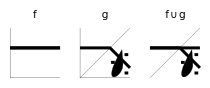
\includegraphics[clip, width=\textwidth]{equality.pdf}}
\caption{Two \label{abuse} functions $f,g$ with $\invlim{f\cup g}=\invlim{f}\cup\invlim{g}$}
\end{figure}

\begin{figure}[h]
\centering{
\includegraphics[clip, width=\textwidth]{strictly.pdf}}
\caption{Two \label{strictly} functions $f,g$ with $\invlim{f\cap g}\supset\invlim{f}\cup\invlim{g}$}
\end{figure}

\begin{figure}[h]
\centering{
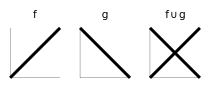
\includegraphics[clip, width=\textwidth]{cross.pdf}}
\caption{Two \label{strictsuperset} functions $f,g$ with $\invlim{f\cap g}\supset\invlim{f}\cup\invlim{g}$}
\end{figure}

\begin{figure}[h]
\centering{
\includegraphics[clip, width=\textwidth]{hilbcross.pdf}}
\caption{Diagramatic representation of\label{cantorfan} $\invlim{f\cup
    g}$ with $f,g$ as defined in figure~\ref{strictsuperset} taking the
  form of a Cantor fan; $\invlim{f}$ and $\invlim{g}$ shown in red}
\end{figure}

\begin{figure}[h]
\centering
\includegraphics[width=6in]{drawing.pdf}
\caption[width=\textwidth]{Diagramatic illustration of 
  \label{drawing} $\invlim{f}$, where $f(x) = \begin{cases}
    \lbrace a\rbrace & x\neq b\\
    \lbrace a,b\rbrace & x=b\\
    \end{cases}$ for some $a,b\in[0,1]$, $a\neq b$}
\end{figure}

\bibliographystyle{unsrt}
\bibliography{references}
\end{document}
